\documentclass[border=10pt]{standalone}
\usepackage[T1]{fontenc}
\usepackage[utf8]{inputenc}
\usepackage[scaled=0.95]{helvet}
\renewcommand{\familydefault}{\sfdefault}
\usepackage{xcolor}
\definecolor{terracotta}{HTML}{C2410C}
\definecolor{sarcelle}{HTML}{0F766E}
\definecolor{violet}{HTML}{7C3AED}
\definecolor{encre}{HTML}{1C1917}
\definecolor{gris}{HTML}{78716C}
\definecolor{grisclair}{HTML}{F5F5F4}
\definecolor{ambre}{HTML}{B45309}
\usepackage{tikz}
\usetikzlibrary{positioning,arrows.meta,fit,backgrounds,calc}
\tikzset{
  boite/.style={draw=#1,fill=#1!7,rounded corners=4pt,align=center,minimum height=1cm,text width=2.9cm,line width=0.8pt,text=encre},
  boite/.default=gris,
  titre/.style={font=\small\bfseries,text=#1},
  fleche/.style={-{Stealth[length=2.6mm]},line width=0.8pt,color=gris},
}
\color{encre}

\begin{document}
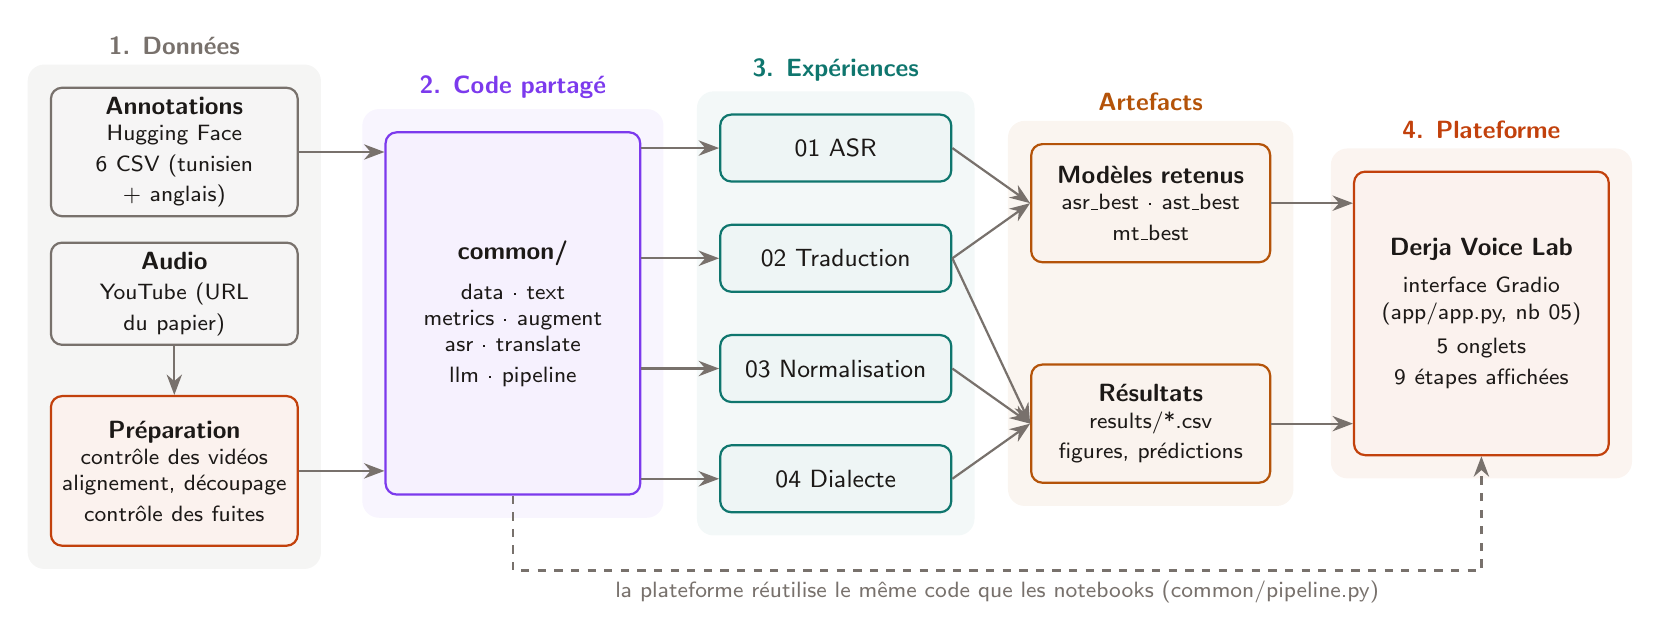
\begin{tikzpicture}[font=\small]
% 1. Données
\node[boite=gris] (hf) at (0,2.3) {\textbf{Annotations}\\\footnotesize Hugging Face\\\footnotesize 6 CSV (tunisien + anglais)};
\node[boite=gris] (yt) at (0,0.5) {\textbf{Audio}\\\footnotesize YouTube (URL du papier)};
\node[boite=terracotta,minimum height=1.9cm] (prep) at (0,-1.75) {\textbf{Préparation}\\\footnotesize contrôle des vidéos\\\footnotesize alignement, découpage\\\footnotesize contrôle des fuites};
% 2. Socle
\node[boite=violet,text width=3.0cm,minimum height=4.6cm] (common) at (4.3,0.25) {\textbf{common/}\\[5pt]\footnotesize data · text\\\footnotesize metrics · augment\\\footnotesize asr · translate\\\footnotesize llm · pipeline};
% 3. Notebooks
\node[boite=sarcelle,text width=2.7cm,minimum height=0.85cm] (nb1) at (8.4,2.35) {01 ASR};
\node[boite=sarcelle,text width=2.7cm,minimum height=0.85cm] (nb2) at (8.4,0.95) {02 Traduction};
\node[boite=sarcelle,text width=2.7cm,minimum height=0.85cm] (nb3) at (8.4,-0.45) {03 Normalisation};
\node[boite=sarcelle,text width=2.7cm,minimum height=0.85cm] (nb4) at (8.4,-1.85) {04 Dialecte};
% Artefacts
\node[boite=ambre,text width=2.8cm,minimum height=1.5cm] (mod) at (12.4,1.65) {\textbf{Modèles retenus}\\\footnotesize asr\_best · ast\_best\\\footnotesize mt\_best};
\node[boite=ambre,text width=2.8cm,minimum height=1.5cm] (res) at (12.4,-1.15) {\textbf{Résultats}\\\footnotesize results/*.csv\\\footnotesize figures, prédictions};
% 4. Plateforme
\node[boite=terracotta,text width=3.0cm,minimum height=3.6cm] (app) at (16.6,0.25) {\textbf{Derja Voice Lab}\\[4pt]\footnotesize interface Gradio\\\footnotesize (app/app.py, nb 05)\\[3pt]\footnotesize 5 onglets\\\footnotesize 9 étapes affichées};
% flèches
\draw[fleche] (hf) -- (hf -| common.west);
\draw[fleche] (yt) -- (prep);
\draw[fleche] (prep.east) -- (prep -| common.west);
\foreach \n in {nb1,nb2,nb3,nb4} \draw[fleche] (common.east |- \n) -- (\n.west);
\draw[fleche] (nb1.east) -- (mod.west);
\draw[fleche] (nb2.east) -- (mod.west);
\draw[fleche] (nb2.east) -- (res.west);
\draw[fleche] (nb3.east) -- (res.west);
\draw[fleche] (nb4.east) -- (res.west);
\draw[fleche] (mod.east) -- (mod -| app.west);
\draw[fleche] (res.east) -- (res -| app.west);
\draw[fleche,dashed] (common.south) -- ++(0,-0.95) -| (app.south) node[pos=0.25,below,font=\footnotesize,text=gris] {la plateforme réutilise le même code que les notebooks (common/pipeline.py)};
% bandeaux
\begin{scope}[on background layer]
\node[fit=(hf)(yt)(prep),fill=grisclair,rounded corners=6pt,inner sep=8pt,label={[titre=gris]above:1. Données}] {};
\node[fit=(common),fill=violet!5,rounded corners=6pt,inner sep=8pt,label={[titre=violet]above:2. Code partagé}] {};
\node[fit=(nb1)(nb4),fill=sarcelle!5,rounded corners=6pt,inner sep=8pt,label={[titre=sarcelle]above:3. Expériences}] {};
\node[fit=(mod)(res),fill=ambre!6,rounded corners=6pt,inner sep=8pt,label={[titre=ambre]above:Artefacts}] {};
\node[fit=(app),fill=terracotta!6,rounded corners=6pt,inner sep=8pt,label={[titre=terracotta]above:4. Plateforme}] {};
\end{scope}
\end{tikzpicture}
\end{document}
